\begin{figure}[h]
	\centering
	\missingfigure{Sequenzdiagramm}		
	\caption{Sequenzdiagramm - A}
	\label{fig:sequenz-a}
\end{figure}


\begin{tcolorbox}
Das dynamische Verhalten des Systems wird mittels Sequenzdiagrammen modelliert.
Hier müssen wahrscheinlich geräteübergreifende Aufrufe modelliert werden.
Findet dafür eine geeignete Notation und nutzt diese durchgehend! 
Achtet weiterhin darauf, dass die anderen Methoden im Klassendiagramm zu finden sind.
Manche Sequenzen erfordern sicherlich eine kurze schriftliche Beschreibung.
\end{tcolorbox}

In diesem Kapitel sind die Sequenzdiagramme beschrieben, die Vorgänge beschreiben bei denen das Verhalten nicht trivial ist.
Nicht trivial ist ein Verhalten bei dem das Diagramm nicht einem ``durchreichen'' von Aufrufen entspricht.
 
\section{Bilder in der App übermitteln}
Das folgende Sequenzdiagramm beschreibt den Vorgang des erfolgreichen Übermitteln eines \\Zählerstandes als Bild.
Zuerst läd der Nutzer ein Foto hoch, dieses wird mittels der Methode azureAnalyse vom Netzwerk-Controller per Post-Request ans Backend der Website geschickt. Dieses leitet das Bild per HTTP an die Klassifizierungsschnittstelle des AzureWrappers weiter. Nach der Antwort wird über HTTP das Bild an die nächste Schnittstelle Area-Detect geschickt. Als letztes wird das Bild noch per HTTP an die Schnittstelle Parse-Text geschickt. Die erhaltenenen Daten werden jetzt einer ersten Plausibilitätsprüfung unterzogen. (Richtigkeit der Stellen und Klassifizierung) \\
Nun wird mittels getUsersMeters() alle Zähler für den Nutzer von der Datenbank abgefragt, um zu Prüfen, ob die Nummer des Zählers in enthalten ist.
Wenn dies der Fall ist wird eine HTTP Response an den Network-Controller gesendet, die die gelesene Zählernummer und den gelesenen Zählerstand übermittelt. Nun wird der Nutzer aufgefordert den gelesenen Wert zu bestätigen. \\
Die Bestätigung entspricht dabei einer manuellen Eingabe.
\begin{figure}[H]
	\centering
	\caption{Erfolgreiche Bildübermittlung}
	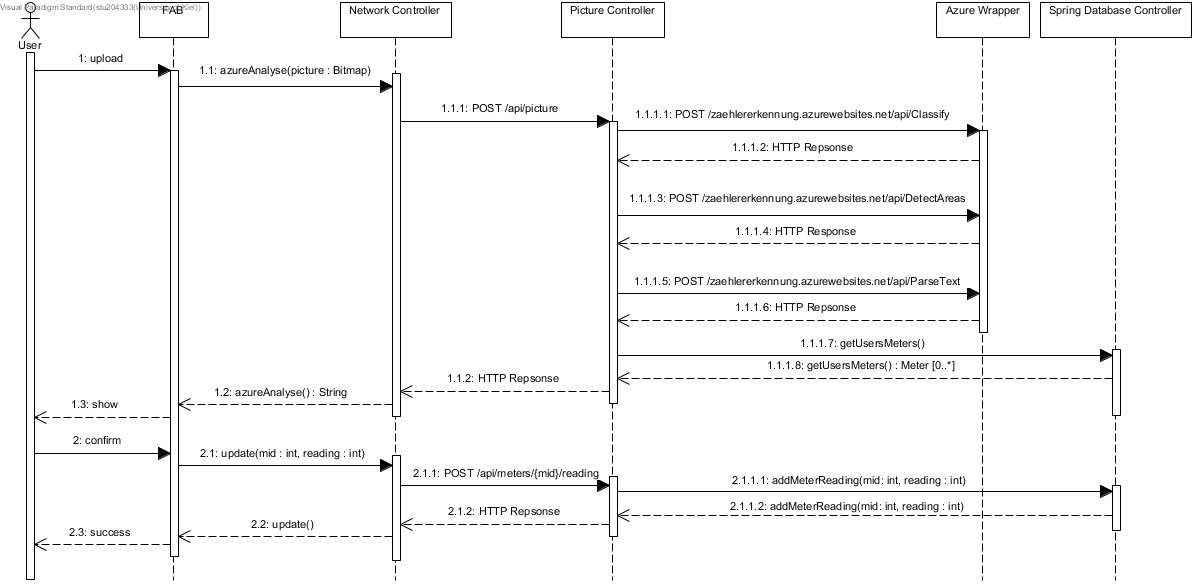
\includegraphics[width=16cm]{img/diagrams/SubmitFotoSequence}
\end{figure}


\section{Zählerstände für User updaten}
Administratoren können unter angabe eines Grundes Zählerstände aktualisieren.
Dafür muss der Administrator zuerst mittels einer HTTP-Requests zu einer Userid alle Zähler vom User Controller abfragen. Danach wird mittels einer weiteren Anfrage alle Zählerstände des Zählers abgefragt. Nun kann mittels eines PUT-request mit der rid ein bestimmter Eintrag verändert werden. Dafür wird der neue Zählerstand, der Grund der Änderung und die Id des Admins versendet, die dann für den Aufruf ''updateReading'' verwendet wird. Wenn die Änderung erfolgreich war sendet der Reading Controller in der HTTP Response einen Erfolg zurück.